\clearpage
\section{常微分方程}
\setstretch{1.75}


\subsection{方程类型速查}

考试中的解方程题目不会超出书上方程类型的范围.
希望以下的整理将有助于同学们复习自查，并在考场上快速回忆出题目对应的方程类型.


\subsubsection{分离变量法}

(1) \textbf{变量分离方程}：形如$f(x) ~\d x = g(y)~\d y$. \textbf{提示}：两边积分.

(2) \textbf{线性替换}：形如$y' = f(ax+by+c)$. \textbf{提示}：令$u = ax+by+c$.

(3) \textbf{齐次函数方程}：形如$y' = f \left( \frac{y}{x} \right)$. \textbf{提示}：令$u= \frac{y}{x}$.

(4) \textbf{豪华版齐次函数方程}：形如$y' = f \left( \frac{a_1 x+ b_1 y + c_1}{a_2 x + b_2 y + c_2} \right)$.
\textbf{提示}：通过线性替换消去分式中的常数$c_1$和$c_2$，化为齐次函数方程.

\subsubsection{全微分方程}

(1) \textbf{全微分方程}：$P(x,y)~\d x + Q(x,y)~\d y =0$，其中左侧的微分形式具有原函数$u(x,y)$.
\textbf{判定方法}：$\frac{\partial Q}{\partial x} = \frac{\partial P}{\partial y}$.
~\textbf{提示}：瞪眼法/偏积分法/线积分法. \vspace{0.25em}

(2) \textbf{假装是全微分方程}：$M(x,y)~\d x + N(x,y)~\d y = 0$，但不符合全微分方程的条件.
\textbf{提示}：a.凑积分因子；b. 移项整理，可能是其他方程类型.

\subsubsection{降阶法}

(1) \textbf{不显含未知函数$y$的方程}：$F(x,y',y'')=0$.
\textbf{提示}：令$z = y'$. 

(2) \textbf{不显含自变量$x$的方程}：$F(y,y',y'')=0$.
\textbf{提示}：令$p = y'$，$y'' = p \frac{\d p}{\d y}$.

\subsubsection{线性方程}

(1) \textbf{一阶线性方程（齐次/非齐次）}：$y' + P(x)y = Q(x)$.
\textbf{提示}：a. 直接背公式；b. 先用变量分离法解对应的齐次方程，再用常数变易法.

(2) \textbf{伯努利方程}：$y' + P(x)y = Q(x)y^{\alpha}$.
\textbf{提示}：令$z = y^{1-\alpha}$，化为一阶线性方程.

(3) \textbf{二阶线性常系数齐次线性方程}：$y'' + py' + q =0$.
\textbf{提示}：特征根法. 需记忆特征根与特解形式的关系（书上表格）. 

(4) \textbf{二阶线性常系数齐次线性方程}：$y'' + py' + q = f(x)$.
\textbf{提示}：先解对应的齐次方程，再加上非齐次方程的任意一个特解.
找特解一般要先猜特解形式，再用待定系数法确定.
需要背诵书上$f(x)$与特解形式的表格（书上说不用背，别信）.
如$f(x)$的形式不在表格中，可用常数变易法.

(5) \textbf{$n$阶线性常系数齐次线性方程}.
\textbf{提示}：特征根法. 需记忆特征根与特解形式的关系（书上表格）.

(6) \textbf{欧拉方程}：
$a_0 x^{n} y^{(n)} + a_1 x^{n-1} y^{(n-1)}+ \cdots + a_{n-1} xy' + a_n y = 0$.
\textbf{提示}：令$x = e^t$.

(7) \textbf{常系数线性微分方程组}.
\textbf{提示}：a.消元法；b. 矩阵解法（非课内）.

\subsection{复习要点} \par



\subsubsection{对于基本概念的补充}\par

\textbf{常微分方程}，是指联系自变量$x$，未知的一元函数$y = y(x)$及其导数的一种函数方程.
若方程中最高含有$n$阶导，则称为\textbf{$n$阶常微分方程}.

类似以下两种形式的方程貌似复合常微分方程的定义，但我们一般不称之为常微分方程：
\begin{eq1}
    y'(x) = y(y(x)) \\
    y'(x) = y(x-1)
\end{eq1} 

满足常微分方程的函数$y(x)$称为该方程的\textbf{解}.
解所对应的图像称为\textbf{积分曲线}.
一个常微分方程通常有无穷多的解，
其中绝大多数呈现一定的规律或结构，从而可以用统一的函数表达式写出来，
并在函数表达式中引入一些任意常数$C$.
对于$n$阶常微分方程，当解的函数表达式中包含了$n$个相互独立的任意常数$C_1,C_2,\cdots C_n$时，
它就能代表该方程的绝大多数解，我们称之为\textbf{通解}.
当$C$变化时，通解对应了一系列积分曲线，或称为一个积分曲线簇.
如果通解不是以$y = y(x)$这种显式表达式给出，而是由隐函数方程的形式给出，则也称为\textbf{通积分}.

“任意常数”这个概念容易让人误以为$C$可以取遍任意实数.
实则不然.
比如下面这个例子：
\begin{eq1}
    x ~\d y -(y  + \sqrt{x^2 + y^2})~\d x = 0
\end{eq1}

它的通解是$y = \frac{1}{2}(Cx^2 - \frac{1}{C})$.
此处需限定$C>0$，因为容易验证当$C<0$时这个表达式不是方程的解.
从这个例子中看出，$C$有时不能取遍任意实数，而只能在一定的范围内任取.
在解微分方程时，一般不需要特别指出$C$的范围.

通过取定通解中的任意常数$C$，使得这个解变成一个确定的函数，就称为方程的\textbf{特解}.
在解方程时，我们一般不会满足于只找到方程的一个特解，而是尽量去求出通解.
不过，要是能直接通过方程“目测”出方程的一个特解，对于解方程也会很有帮助的.

微分方程的通解有时就是全部的解（例如线性微分方程），但有时却不是.
不包括在通解之中的解称为\textbf{奇解}（因此奇解一般不说是一个特解）.
考虑教材9.2节的例2：
\begin{eq1}
    \frac{\d y}{\d x} = \sqrt[4]{y^3}
\end{eq1}

它的通解是$y = \frac{1}{256}(x+C)^4$，$x \ge -C$.
同时，$y = 0$显然也是该方程的一个解，但并不在通解之中，因此是奇解.
可以看到奇解有一个极其特殊的性质，就是它处处与通解所对应的积分曲线簇相切.
更直观地说，如果考虑通解的积分曲线簇“扫过”的区域，那么奇解就描出了这个区域的轮廓.
即：奇解恰好构成了通解的\textbf{包络}.

在高等数学的范围内，我们没有一般性的手段来判断一个微分方程有没有奇解和有多少奇解.
因此微分方程的题目理论上不会有解出“所有解”的要求，只要解出通解就算完成任务.
如果一定需要解出奇解，可以回溯自己解出通解的过程——某些不严谨的步骤中往往可以揪出奇解来.
例如上面举出的方程，第一步需对其进行分离变量：
\begin{eq1}
    \d x = y^{\frac{4}{3}}~\d y
\end{eq1}

这一步两边除以了$\sqrt[4]{y^3}$，问题在于没有考虑$y=0$的情况.
这正是被遗漏掉的奇解.
反过来说，如果题目只要求解出通解，那么在计算过程中就不需要在意$y$是否等于$0$这种细枝末节了.
因为遗漏掉少数一两个解不可能影响通解的形式.

\subsubsection{*微分方程解的存在和唯一性定理}\par

微分方程解的存在和唯一性定理不需要掌握证明细节，但需要知道构造皮卡序列的原理.

在微分方程通解的基础上，如果再给定一些\textbf{初值条件}，就能确定通解中的一些任意常数，从而减少解的数量.
初值条件可以是一个指定点处的函数值，或者各阶导数的值.
一般情况下，$n$阶微分方程如果给出了$n$个初值条件，就可以确定唯一解.
像这种通过微分方程+初值条件确定唯一特解的问题，叫做\textbf{初值问题}或\textbf{柯西问题}.

本节将要探讨一阶初值问题：\vspace{0.5em}
$$
\setstretch{1.25}
    \begin{cases}
        y' = f(x,y(x))\\
        y(x_0) = y_0
    \end{cases} 
$$ 
\setstretch{1.75}

该问题与以下的积分方程等价（按书上写法）：
\begin{eq1}
    y = y_0 + \int_{x_0}^{x} f(x,y(x))\,\d x 
\end{eq1}

为了避免积分变量与$x$混淆，也可写成：
\begin{eq1}
    y = y_0 + \int_{x_0}^{x} f(\tau,y(\tau))\,\d \tau 
\end{eq1}

等号右侧可视为一个积分算子$T$，
它将一个函数$y(x)$映射为一个新的（关于$x$的）函数
$y_0 + \int_{x_0}^{x} f(\tau,y(\tau))\,\d \tau$，
将其记为$T[y(x)]$.
则上述积分方程可以记为：
\begin{eq}
    y(x) = T[y(x)]
\end{eq}

这说明满足方程的函数$y(x)$是映射$T$的\textbf{不动点}.
换句话说，$y(x)$在被$T$映射后是保持不变的.
这种看待问题的方式很新，
不过我们曾经在数列极限中碰到过类似的问题.
为了类比，我们回顾以下的问题.
假设数列$\left\{ x_n \right\}$由以下的递推公式给出：
\begin{eq}
    x_{n+1} = f(x_{n})
\end{eq}

其中$f(x)$为连续函数，并假设$\left\{ x_n \right\}$极限等于$x^{*}$.
我们可以对递推公式两侧同时取$n \to \infty$的极限，得到：
\begin{eq}
    x^{*} = f(x^{*})
\end{eq}

这说明$x^{*}$是函数$f(x)$的不动点.
反过来说，为了求解不动点方程$x = f(x)$，
可以构造数列$x_{n+1} = f(x_{n})$，
在一定条件下证明该数列的极限$x^{*}$存在（且唯一）.
这样一来，也就相当于证明了不动点方程的解存在唯一，
并且可以利用数列$\left\{  x_n \right\}$数值逼近$x^{*}$.

我们借鉴上述的思路来解决函数方程$y(x) = T[y(x)]$.
利用映射$T$做递推，定义一个函数列$\left\{y_n (x)\right\}$满足$y_{n+1}(x) = T[y_n (x)]$.
这就是\textbf{皮卡序列}.
假设皮卡序列收敛，即函数列$\left\{ y_n (x) \right\}$趋向于一个确定的函数$y^{*}(x)$，
那么通过对递推公式两侧取极限可知，
这个$y^{*}(x)$就满足$y^{*}(x) = T[y^{*}(x)]$.
这也就是原初值问题的唯一解.

上述推理的漏洞在于，我们只是假设了皮卡序列收敛，而事实上这不一定成立.
因此，我们需要在现有理论“雏形”的基础上再加以一定条件的限制，
才能使之成为教材上的定理.
应该加什么样的条件呢？
我们再次回到一元函数不动点问题的类比上.
图1展示了高中常用的找递推数列极限的“蛛网图”.
可以直观地看出，如果函数$f(x)$是比较“平缓”的曲线，
那么$f(x)$与$y=x$就能有唯一的交点，即$f(x)$有唯一的不动点.

现在的问题在于用什么样的条件可以保证$f(x)$足够“平缓”.
比较容易想到的是用$|f'(x)|<1$来限制$f(x)$的斜率，不过这样就额外要求$f(x)$可导，条件太苛刻了.
这里我们采用\textbf{压缩映射}作为关键的条件，
即在给定范围内，$f(x)$满足：对任意的$x_1$和$x_2$，
存在常数$L \in (0,1)$，
使得$|f(x_1) - f(x_2)| \le L|x_1 - x_2|$.
这个条件是在说，任意两点$x_1$和$x_2$被$f$映射过后，距离缩短.
因此“压缩映射”是一个很形象的名称.
\textbf{压缩映射原理}指出，如果一个数列是由压缩映射来递推定义的，
那么它收敛于压缩映射的不动点.

回到皮卡序列收敛的问题.
延续刚才的思路，我们将压缩映射原理推广到对于函数列的讨论上.

\begin{figure}[H] 
    \centering
    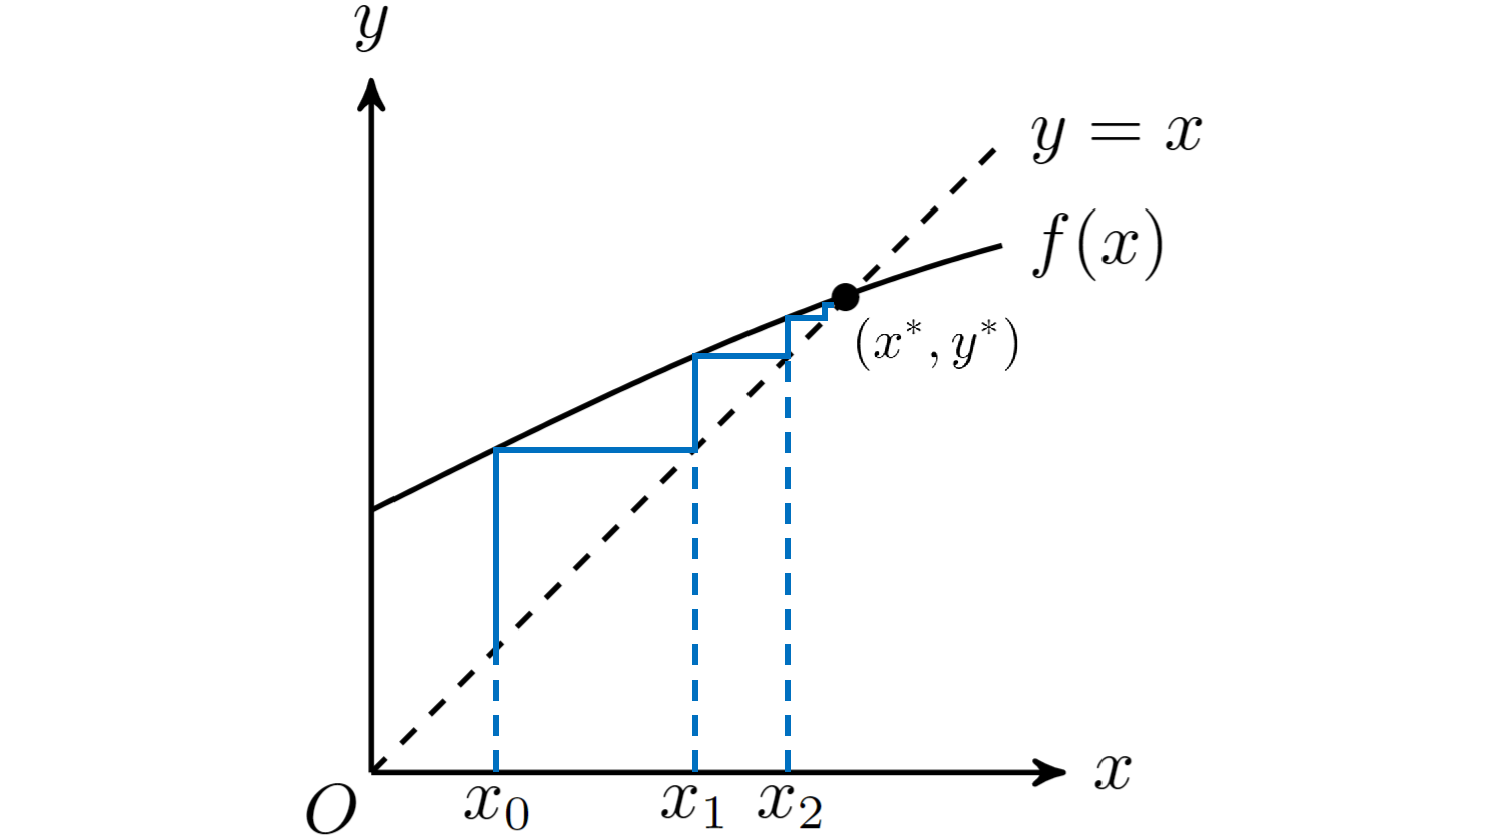
\includegraphics[width=0.5\textwidth]{fig9-1.png}
    \caption{构造递推数列$x_{n+1} = f(x_n)$逼近不动点} 
\end{figure}


我们定义$[a,b]$上两个连续函数$y_1(x)$和$y_2(x)$的距离为：
\begin{eq1}
    d(y_1(x),y_2(x)) = \max\limits_{a \le x \le b} \left| y_1(x) - y_2(x) \right|
\end{eq1}

如果说$T$是一个对函数的压缩映射，也就是说存在常数$L_1 \in (0,1)$，使得：
\begin{eq1}
    d\left(T[y_1(x)],T[y_2(x)] \right) \le L_1 \cdot d \left( y_1(x),y_2(x) \right)
\end{eq1}

现在我们再来看教材上关于微分方程解的存在唯一性的关键条件——
\textbf{Lipschitz条件}.
即，存在常数$L$，使得函数$f(x,y)$在定义域$D$内满足：
\begin{eq1}
    |f(x,y_1) - f(x,y_2)| \le L |y_1 - y_2|,~~(x,y_i) \in D,~~i = 1,2    
\end{eq1}

这个条件正是使得积分算子$T$成为压缩映射的条件.
事实上，若$f(x,y)$的定义域是闭矩形域$R: |x-x_0| \le a ,~|y - y_0 | \le b$时，我们有：
\begin{eq1}
    d \left( T[y_1(x)],T[y_2(x)] \right) 
    &= \max\limits_{|x - x_0| \le h} \left| \int_{x_0}^{x} f(x,y_1(x)) -  \int_{x_0}^{x} f(x,y_2(x))\right| \\
    &\le h \cdot \max\limits_{|x - x_0| \le h} 
    \left|  f(x,y_1(x)) - f(x,y_2(x)) \right| \\
    &\le Lh \cdot \max\limits_{|x - x_0| \le h} |y_1(x) - y_2(x)| \\
    &= Lh \cdot d \left( y_1(x) - y_2(x) \right)
\end{eq1}

注意，虽然$x \in (x_0 -a , x_0 + a)$，但是不能保证该区间一定存在解.
因此在上面的计算中我们没有简单地限定$|x-x_0|< a$，
而是另设了区间半径$h$.
可以发现，当$Lh<1$，即$h < \frac{1}{L}$时，$T$是压缩映射.
根据压缩映射原理（Banach不动点定理），
不动点是存在唯一的，
它也正是初值问题的唯一解.
按这个思路来构建证明过程，存在性和唯一性就可以由压缩映射来保证，不需要额外证明了.

\subsubsection{*线性微分方程解的结构}\par

本章着重讨论了线性微分方程.
由于大多数同学还没有学线性代数，
对于“线性”的概念还比较模糊
（当然有可能学了还是感觉模糊QAQ）.
这直接影响到对于线性微分方程解的结构的理解.
希望本节的讲解有助于大家直观地“看见”线性微分方程的解，
从而轻松地记忆线性微分方程的各种性质.

说到“线性”，我们更熟悉的是线性代数方程，也就是所谓“$n$元一次方程”.
下面是一个“三元一次方程”的例子：
\begin{equation}
    \setlength\abovedisplayskip{4pt}
    \setlength\belowdisplayskip{4pt}
    \begin{aligned}
    x_1 - 2 x_2 + x_3 = 0
    \end{aligned}
\end{equation}

像$(1)$这种只含线性项，不含常数项的线性方程，称为$\textbf{齐次方程}$.
如果在此基础上保持线性项不动，将常数项变为非零，就成为了一个对应的$\textbf{非齐次方程}$.
例如，$(1)$对应的一个非齐次方程是：
\begin{equation}
    \setlength\abovedisplayskip{4pt}
    \setlength\belowdisplayskip{4pt}
    \begin{aligned}
    x_1 - 2 x_2 + x_3 = 2
    \end{aligned}
\end{equation}

我们知道，$(1)$和$(2)$其实是空间平面的方程.
将两个平面分别记为$S_1$和$S_2$，则它们同时表示两个方程的解集.
二者是相互平行的.
与非齐次方程$(2)$相比，齐次方程$(1)$的特殊之处在于，它所对应的平面$S_1$经过原点.
显然，上面的两个方程都有无穷多解，但是也并非任何$\mathbb{R}^3$向量都是解.
接下来我们借助上述的几何图像来研究线性代数方程解的结构.

对于齐次方程$(1)$，我们任取平面$S_1$上两个不共线的向量
$\bm{v}_1 = (1,1,1)$和$\bm{v}_2 = (2,1,0)$.
当然，它们是齐次方程$(1)$的两个\textbf{线性无关的特解}.
根据平面向量分解定理，
平面上的任意向量$\bm{v}$都可以由$\bm{v}_1$和$\bm{v}_2$线性组合而成.
这就是说，对任意$\bm{v} \in S_1$，总存在合适的一组系数$C_1,C_2 \in \mathbb{R}$，
使得$\bm{v} = C_1 \bm{v}_1 + C_2 \bm{v}_2$.
反过来说，若设$C_1$和$C_2$为任意常数，
则$\bm{v} = C_1 \bm{v}_1 + C_2 \bm{v}_2$就表达出了$(1)$的所有解，
也就是\textbf{通解}.
可见，\textbf{齐次方程的通解是由一些线性无关特解的任意线性组合}.

知道了齐次方程$(1)$解的结构，$(2)$的解很容易表示.
从图像上看，$S_2$是$S_1$向上平移$2$单位得到的.
也就是说，$(1)$的任意一个解$\bm{v} \in S_1$向上平移$2$单位就成为了$(2)$的解，即$\bm{v} + \bm{w^{*}} \in S_2$.其中$\bm{w^{*}}=(0,0,2)$本身也是$(2)$的一个解. 
反过来，设$C_1$和$C_2$为任意常数，
则$\bm{w} = C_1 \bm{v}_1 + C_2 \bm{v}_2 + \bm{w^{*}}$就表达出了$(1)$的所有解，即$(2)$的通解.
同时还可以发现，上述通解的结构与$\bm{w^{*}}$的具体取法是无关的，只要它是非齐次方程$(2)$的特解即可.
据此，我们可以说：\textbf{非齐次方程的通解 = 对应齐次方程的通解 + 任意一个非齐次方程的特解}.而且，\textbf{任意两个非齐次方程的特解相减，会得到对应齐次方程的特解}.\vspace{0.5em}

现在我们来回答关键的问题：线性代数方程与线性微分方程之间有什么共同之处吗？
相信同学们已经看出：不仅有，而且非常多.
事实上，上文中用\textbf{粗体字}打出的概念和结论，
与我们在线性微分方程中使用和提出的完全一致，不需要丝毫变动.
简单地举个例子. 考虑以下的二阶线性常系数方程：
\begin{equation}
    \setlength\abovedisplayskip{4pt}
    \setlength\belowdisplayskip{2pt}
    y'' - y = 0  \tag{1}
\end{equation}
\begin{equation}
    \setlength\abovedisplayskip{2pt}
    \setlength\belowdisplayskip{4pt}
    y'' - y = 2  \tag{2}
\end{equation}

对于齐次方程$(1)$，用特征根法容易找到它的两个线性无关特解$\bm{v}_1 = e^x$，$\bm{v}_2 = e^{-x}$.
而非齐次方程$(2)$的一个特解是$\bm{w^{*}} = -2$.
这里特意将微分方程的特解也用粗体字母表示，
意在表明它们可以完全类比于向量.

线性代数方程和线性微分方程之所以表现得如此相似，
根本原因在于它们的解集都具有一种\textbf{对于线性组合封闭}的性质.
这意思是说，如果$\bm{v}_1$和$\bm{v}_2$都是某个齐次线性方程（不论代数方程还是微分方程）的解，则$C_1 \bm{v}_1 + C_2 \bm{v}_2$一定也是该齐次方程的解.
具有这种性质的空间称为\textbf{线性空间}.
它就是线性代数的研究对象.
本节所谈的关于两种线性方程解的问题，
是在讨论线性空间的普遍性问题
（即解与解之间线性组合的关系），
并不涉及到“向量”与“函数”作为不同数学对象的特殊性问题.
因此，
如果利用线性空间来讨论线性方程的解，
实际上没有必要区分是线性代数方程的解（向量）还是线性微分方程的解（函数）.
同学们可以尝试用这种方式理解我接下来提出的定义和结论：\vspace{0.5em}

\textbf{定义}~~\textit{如果一个线性空间有$n$个基向量，即由至少$n$个向量才可以线性组合成该空间内任意的向量，则称这个线性空间是$\textbf{$n$维线性空间}$.}

\textbf{例子}~~\textit{我们平常所说的$3$维欧氏空间$\mathbb{R}^3$是一个$3$维线性空间.
其中一个过原点的平面构成$2$维线性空间.}

\textbf{引理}~~\textit{设$S$为$n$阶齐次线性微分方程的解集，
则$S$是$n$维线性空间.}


\subsection{解题方法}

解微分方程的关键在于准确判断方程的类型.
但考试题目可能不会像课本例题那样容易识别，需要经过一些变换才能看出来.
包括：(1)对方程进行移项整理；(2)把$x$看成关于$y$的函数；$(3)$凑微分.\par
~\par

\begin{example}
    {1}{
        \textit{解微分方程：$(x^3 + 2y)~\d x = x~\d y$}.
    }
\end{example}
\begin{remark}
    整理后发现该方程是一阶线性方程.
\end{remark}
\begin{solution}
    整理得到：
    \begin{eq1}
        y' - \frac{2}{x} y = x^3
    \end{eq1}

    此为一阶线性非齐次方程，
    可以套用公式，或者通过先解对应齐次方程再用常数变易法，
    求得通解：
    \begin{eq1}
        y = x^3 + Cx^2
    \end{eq1} \qed \par
\end{solution}
~\par

\begin{example}
    {2(2023)}{
        求方程$(xy -x^3y^3)~\d x + (1+x^2)~\d y = 0$满足条件$y(0)=1$的解.
    }
\end{example}
\begin{remark}
    整理后发现该方程是伯努利方程（如果没看出来的话则会变成白努力方程（被打））.
\end{remark}
\begin{solution}
    改写方程的形式：
\begin{eq1}
    y' + \frac{x}{1+x^2}\cdot y = \frac{x^3}{1+x^2} \cdot y^3
\end{eq1}

做换元$u = y^{-2}$，则$u' = -2y^{-3}y'$. 代入得：
\begin{eq1}
    u' - \frac{2x}{1+x^2}\cdot u = \frac{-2x^3}{1+x^2}
\end{eq1}

此为一阶线性方程，可以套用公式，或者通过先解对应齐次方程再用常数变易法，求得通解：
\begin{eq1}
    y^{-2} = u = C(1+x^2) - (1+x^2) \ln (1+x^2) -1
\end{eq1}

代入初值条件$y(0) = 1$，解得$C=2$.
故满足条件的解为：
\begin{eq1}
    y = \frac{1}{\sqrt{2x^2 + 1 - (1+x^2) \ln (1+x^2)}}
\end{eq1} \qed \par
\end{solution}
~\par

\begin{example}
    {3}{
        求微分方程$(x^3 - y^2)~\d x + (x^2 y + xy)~\d y = 0$的通解.
    }
\end{example}
\begin{remark}
    仅通过简单的移项无法将方程转化为已知的方程类型.
    此题需要凑微分.
\end{remark}

\textbf{解答I}~~凑微分$2y ~\d y = \d y^2$.
令$u = y^2$. 则原方程化为：
\begin{eq1}
    \frac{\d u}{\d x} = \frac{2u}{x^2 + x} - \frac{2x^2}{x^2 + 1}
\end{eq1}

这个线性方程的通解为：
\begin{eq1}
    \left( \frac{1+x}{x}\right)^2 u + (1+x)^2 = C
\end{eq1}

即：
\begin{eq1}
    \left( \frac{1+x}{x}\right)^2 y^2 + (1+x)^2 = C
\end{eq1} \qed \par \vspace{0.5em}

\textbf{解答II}~~原方程可化为：
\begin{eq1}
    x~\d x + y~\d y + y \cdot \frac{x~\d y - y ~\d x}{x^2} = 0
\end{eq1}

即：
\begin{eq1}
    \frac{1}{2} \d (x^2 + y^2) + y ~\d ~ \left( \frac{y}{x} \right) = 0
\end{eq1}

两边同时除以$\sqrt{x^2 + y^2}$，得：
\begin{eq1}
    \frac{1}{2} \cdot \frac{\d (x^2 + y^2)}{\sqrt{x^2 + y^2}} + 
    \frac{1}{\sqrt{1+ (\frac{y}{x})^2}} \cdot \frac{y}{x} \cdot \d ~ \left( \frac{y}{x}\right) = 0
\end{eq1}

即：
\begin{eq1}
    \d ~ \left( \sqrt{x^2 + y^2} \right) + 
    \d ~ \left( \sqrt{1 + \left( \dfrac{y}{x} \right)^2 } \right) = 0
\end{eq1}

故：
\begin{eq1}
    \sqrt{x^2 + y^2} + \frac{\sqrt{x^2 + y^2}}{x} = C
\end{eq1}

即：
\begin{eq1}
    (1+x)\sqrt{x^2 + y^2} = Cx
\end{eq1} \qed \par
~\par

\begin{example}
    {4}{
        求方程$y' = \frac{y}{x+y^3}$的通解.
    }
\end{example} \vspace{0.5em}

\begin{remark}
    此题形式简单，欲分离变量，但是必须要将$x$视为$y$的函数.
\end{remark}\vspace{0.5em}

\begin{solution}
    原方程化为：
    \begin{eq1}
        \frac{\d x}{\d y} - \frac{1}{y}x = y^2
    \end{eq1}

    此为关于$x=x(y)$的一阶线性非齐次方程. 通解为：
    \begin{eq1}
        x = y \left( \frac{y^2}{2}+C \right)
    \end{eq1} \qed \par 
\end{solution}
~\par

\begin{example}
    {5}{
        求微分方程$y' + \frac{1}{x} = x e^{-y}$
    }
\end{example}\vspace{0.25em}

\begin{remark}
    用凑微分法处理掉$y$的指数项，转化为线性方程.
\end{remark}\vspace{0.25em}

\begin{solution}
    原方程化为：
    \begin{eq1}
        e^y \frac{\d y}{\d x} + \frac{1}{x} e^y = x
    \end{eq1}
    ，即
    \begin{eq1}
        \frac{\d e^y}{\d x} + \frac{1}{x}e^y = x
    \end{eq1}

    这是关于$e^y$的一阶线性非齐次方程，求得通解为：
    \begin{eq1}
        e^y = \frac{1}{x} \left( \frac{1}{3}x^3 + C \right)
    \end{eq1}

    即：
    \begin{eq1}
        y = \ln \left[ \frac{1}{x} \left( \frac{1}{3}x^3 + C \right) \right]
    \end{eq1} \qed \par
\end{solution} \vspace{0.5em}

\begin{example}
    {6}{
        解微分方程$(x^2 + y^2 + 3)\frac{\d y}{\d x} = 2x \left( 2y - \frac{x^2}{y} \right)$.
    }
\end{example}
\begin{remark}
    通过凑微分转化为齐次方程.
\end{remark}
\begin{solution}
    原方程化为：
    \begin{eq1}
        \frac{y}{x} \cdot \frac{\d y}{\d x} = \frac{2(2y^2 - x^2)}{x^2 + y^2 + 3}.
    \end{eq1}

    令$u = x^2$，$v = y^2$，则原方程化为：
    \begin{eq1}
        \frac{\d v}{\d u} = \frac{2(2v-u)}{u+v+3}
    \end{eq1}

    解方程$2v-u=0$，$u+v+3=0$，得到$u=-2$，$v= -1$，
    再令$U = u+2$，$V = v+1$.
    上述方程化为：
    \begin{eq1}
        \frac{\d V}{\d U}  = \frac{2(2V-U)}{U+V}
    \end{eq1}

    作变量替换$W = \frac{V}{U}$得到：
    \begin{eq1}
        U \frac{\d W}{\d U} = - \frac{W^2 -3W+2}{W+1}
    \end{eq1}

    这是变量分离方程，解得$U(W-2)^3 = C(W-1)^2$，回代得：
    \begin{eq1}
        (y^2 - 2x^2 -3)^3 = C(y^2 - x^2 -1)^2
    \end{eq1} \qed \par
\end{solution}
~\par

以下补充一些更加特殊的例题，供参考.\par
~\par

\begin{example}
    {7(应用题，2022)}{
        假设平面直角坐标系第一象限中有一条曲线 \( L = \{(x, y(x)) \mid x \geq1 0\} \)，
        其中 \( y(0) = 1 \)，\( y(x) \) 是严格递减的、正的、可导函数.
        任取 \( L \) 上一点 \( M \)，\( L \) 在 \( M \) 点的切线交于 \( x \) 轴于点 \( A \)，
        假定从 \( M \) 到 \( A \) 的直线段的长度恒为 1.
        求出 \( y = y(x) \) 所满足的一阶常微分方程，并且解出这个方程的初值问题 \( y(0) = 1 \).
    }
\end{example} \vspace{0.5em}

\begin{solution}
    设 \( M = (x, y(x)) \). 
    曲线 \( L \) 在 \( M \) 点的切线方程为：
    \begin{eq}
        Y - y = y'(x)(X - x) 
    \end{eq}

    此切线与 \( x \) 轴的交点 \( A \) 满足 \( Y = 0 \)，因此：
    \begin{eq}
        0 - y = y'(x)(X - x)
    \end{eq}

解得：
\begin{eq1}
    A = \left(x - \frac{y}{y'(x)}, 0\right)
\end{eq1}

从 \( M = (x, y) \) 到 \( A = \left(x - \frac{y}{y'(x)}, 0\right) \) 的直线段长度为：
\begin{eq1}
    \sqrt{\left(\frac{y}{y'(x)}\right)^2 + y^2} 
\end{eq1}

根据题意，该长度恒为 $1$：
\begin{eq1}
    \sqrt{\left(\frac{y}{y'(x)}\right)^2 + y^2} = 1
\end{eq1}

平方后得到：
\begin{eq1}
    \frac{y^2}{(y'(x))^2} + y^2 = 1
\end{eq1}

整理得：
\begin{eq1}
    (y'(x))^2 = \frac{y^2}{1 - y^2} 
\end{eq1}

由于 \( y(x) \) 严格递减且为正函数，
故 \( y'(x) < 0 \) 且 \( y > 0 \)，因此：
\begin{eq1}
    y'(x) = -\frac{y}{\sqrt{1 - y^2}}
\end{eq1}

这是一阶常微分方程：
\begin{eq1}
    \frac{\d y}{\d x} = -\frac{y}{\sqrt{1 - y^2}} 
\end{eq1}

分离变量并积分：
\begin{eq1}
    -\frac{\sqrt{1 - y^2}}{y} \d y = \d x 
\end{eq1}

令 \( y = \sin t \)，
则 \( \d y = \cos t ~\d t \)，代入得：
\begin{eq1}
    -\frac{\sqrt{1 - \sin^2 t}}{\sin t} \cos t \,& \d t = \d x 
\end{eq1}

整理得：
\begin{eq1}
    -\cot t \cos t \, \d t &= \d x
\end{eq1}

两边积分，解得：
\begin{eq1}
     x = -\sqrt{1 - y^2} + 
    \ln\left(1 + \sqrt{1 - y^2}\right) - \ln y + C
\end{eq1}

代入初值条件 \( y(0) = 1 \)：
\begin{eq1}
    0 = -\sqrt{1 - 1} + \ln(1 +& \sqrt{1 - 1}) - \ln 1 + C \\
    0 = 0 + \ln 1 & - 0 + C \\
    C =& ~0 
\end{eq1}

因此，解为：
\begin{eq1}
    x = -\sqrt{1 - y^2} + \ln\left(1 + \sqrt{1 - y^2}\right) - \ln y
\end{eq1} \qed \par
\end{solution} 
~\par

\begin{example}
    {8(解的存在唯一性定理)}{
        考虑定义在矩形区域$R = \{ (t,x) \in \mathbb{R}^2 \mid |t|\le 1 ,~|x| \le 1 \}$
        上的初值问题：
        \begin{eq1}
            \frac{\d x}{\d t} = x+1,~~~x(0)=0
        \end{eq1}
    }
\end{example}
\textit{(a)根据解的存在唯一性定理，说明该初值问题的解存在且唯一，并给出解的存在区间.} 

\textit{(b)写出该初值问题的皮卡序列，并通过对皮卡序列取极限求出初值问题的解}. \vspace{0.5em}

\textbf{解答}~~

$\bm{(a)}$~~初值问题右端函数$f(t,x)=x+1$在$R$中满足：
\begin{eq1}
    \frac{|f(t,x_1) - f(t,x_2)|}{|x_1 - x_2|} = \frac{|(x_1 + 1) - (x_2 + 1)|}{|x_1 - x_2|} = 1
\end{eq1}

这蕴含着$|f(t,x_1) - f(t,x_2)| \le |x_1 - x_2|$，即$L=1$的Lipschitz条件.
而$f(t,x)$在$R$中的最大值$M=2$.
故$h = \min\{a,\frac{b}{M}\} = \frac{1}{2}$.
因此上述初值问题在$\left[ -\frac{1}{2} , \frac{1}{2} \right] $的解存在且唯一.\vspace{0.5em}

$\bm{(b)}$~~将初值问题改写为积分方程：
\begin{eq1}
    x(t) = x(0) + \int_0^t f(\tau,x(\tau)) ~\d \tau = \int_0^t (x+1) ~\d \tau
\end{eq1}
则皮卡序列有以下递推关系：
\begin{eq1}
    x_n(t) = \int_0^t (x_{n-1}(\tau) + 1) ~\d \tau
\end{eq1}

计算皮卡序列的前几项如下：
\begin{eq1}
    x_0(t) &= 0 \\
    x_1(t) &= \int_0^t (0+1)~\d \tau = t \\
    x_2(t) &= \int_0^t (\tau +1)~\d \tau = t + \frac{t^2}{2} \\
    x_3(t) &= \int_0^t (\tau + \frac{\tau^2}{2}+1)~\d \tau = t + \frac{t^2}{2}+ \frac{t^3}{6} \\
    \cdots
\end{eq1}

由上述计算可知皮卡序列的通项为：
$x_{n}(t) = t + \frac{t^2}{2!} + \frac{t^3}{3!} + \cdots + \frac{t^n}{n!}$.
事实上，若$x_{k}(t)$满足该通项公式，则：
\begin{eq1}
    x_{k+1}(t) &= \int_0^t (x_{k}(\tau)+1)~\d \tau \\
    &= \int_0^t \left( 1 + \tau + \frac{\tau^2}{2!} + \frac{\tau^3}{3!} + \cdots + \frac{\tau^k}{k!} \right)~\d \tau \\
    &= t + \frac{t^2}{2!} + \frac{t^3}{3!} + \cdots + \frac{t^k}{k!} + \frac{t^{k+1}}{(k+1)!}
\end{eq1}

取$n \to +\infty$的极限，并结合$e^t$的泰勒级数，得到初值问题的解：
\begin{eq1}
    x(t) = \lim\limits_{n \to \infty} x_{n}(t)
    &= \lim\limits_{n \to \infty} \left(t + \frac{t^2}{2!} + \frac{t^3}{3!} + \cdots + \frac{t^n}{n!}\right) \\
    &= e^t - 1
\end{eq1} \qed \par
~\par

\begin{example}
    {9}{
        可微函数$f(x)$满足$f'(x) = f(x) + \int_0^1 f(x) ~\d x$，
        且$f(0) = 1$. 求$f(x)$.
    }
\end{example}\vspace{0.5em}

\begin{remark}
    注意方程右侧的定积分虽然也含$f(x)$，但是定积分的值本身只是一个常数而已.
\end{remark}\vspace{0.5em}

\textbf{解答}~~令$\int_0^1 f(x) \d x = a$.
则原方程化为：
\begin{eq1}
    \left(  f(x) - a\right)' = f(x)-a
\end{eq1}

因而可视为关于$f(x)-a$的一阶线性齐次方程. 
其通解为：
\begin{eq1}
    f(x) - a = Ce^x
\end{eq1}

代入初值条件，得：
\begin{eq1}
    f(0) = C-a = 1
\end{eq1}

因此：
\begin{eq1}
    a = \int_0^1 \left( Ce^x -a \right)~\d x = C(e-1)-a
\end{eq1}

解得$a = \frac{e-1}{3-e}$，$C = \frac{2}{3-e}$，即：
\begin{eq1}
    f(x) = \frac{2e^x -e + 1}{3-e}
\end{eq1} \qed \par
~\par

\begin{example}
    {10}{已知微分方程$y'+y = e^{\sin x}$.
        证明：方程存在唯一的以$2\pi$为周期的解.}
\end{example}
\textbf{证明}~~这是一阶线性非齐次方程.
其通解为：
\begin{eq1}
    y(x) = e^{-x} \left( \int_0^x e^{\sin t} e^t ~\d t +C \right)
\end{eq1}

则：
\begin{eq1}
    y(x+2\pi) - y(x) 
    &= e^{-(x+2 \pi)} \left( \int_0^{x+2\pi} e^{\sin t} e^t ~\d t +C \right)
    -e^{-x} \left( \int_0^x e^{\sin t} e^t ~\d t +C \right) \\
    &= e^{-x} \left[
        \left( \frac{1}{e^{2\pi}} - 1 \right)C
        + \frac{1}{e^{2\pi}}\int_0^{x+2\pi} e^{\sin t}e^{t} ~\d t
        - \int_{0}^{x} e^{\sin t}e^{t} ~\d t
    \right]
\end{eq1}

其中：
\begin{eq1}
    \frac{1}{e^{2\pi}}\int_0^{x+2\pi} e^{\sin t}e^{t} ~\d t &=
    \frac{1}{e^{2\pi}} \left( \int_0^{2\pi} e^{\sin t}e^{t} ~\d t +
    \int_{2\pi}^{x + 2\pi} e^{\sin t}e^{t} ~\d t \right) \\
    &= \frac{1}{e^{2\pi}} \left( \int_0^{2\pi} e^{\sin t}e^{t} ~\d t +
    e^{2\pi} \int_{2\pi}^{x + 2\pi} e^{\sin (t - 2\pi)}e^{t - 2\pi} ~\d (t - 2\pi) \right) \\
    &= \frac{1}{e^{2\pi}}  \int_0^{2\pi} e^{\sin t}e^{t} ~\d t
    + \int_0^x e^{\sin u} e^u ~\d u \\
    &= \frac{1}{e^{2\pi}}  \int_0^{2\pi} e^{\sin t}e^{t} ~\d t
    + \int_0^x e^{\sin t} e^t ~\d t
\end{eq1}

代入$y(x+2\pi) - y(x)$的表达式中：
\begin{eq1}
    y(x+2\pi) - y(x) = e^{-x} \left[ \left( \frac{1}{e^{2\pi}} -1 \right) C
    + \frac{1}{e^{2\pi}} \int_{0}^{2\pi} e^{\sin t} e^{t} ~\d t \right] := C_1 e^{-x}
\end{eq1}

$y(x)$以$2\pi$为周期当且仅当$y(x+2\pi) - y(x) = 0$，即：
\begin{eq1}
    C_1 = \left( \frac{1}{e^{2\pi}} -1 \right) C
    + \frac{1}{e^{2\pi}} \int_{0}^{2\pi} e^{\sin t} e^{t} ~\d t = 0
\end{eq1}

解得唯一的$C = \frac{1}{e^{2\pi} -1 } \int_{0}^{2\pi} e^{\sin t}e^t ~\d t$.
故方程存在唯一的以$2\pi$为周期的解. \qed \par